\section{Full protocol and reproducibility}

\paragraph{Dataset composition.} The evaluated intersection contains 177 non-empty traces from 40 benchmark-qualified task groups. Human records are expert terminal inputs; Agent records are structured bash tool calls. Table~\ref{tab:appendix-data} gives the per-suite counts. The source is Cyber Task Horizons, pinned to revision \texttt{178c0da1800f9c07311e1b8d6c61dd8104e7b4ae} under CC BY 4.0. The task label denotes the same CTF challenge, not a shared intrusion or actor.

\begin{table}[t]
\centering
\caption{Composition of the evaluated public trace subset.}
\label{tab:appendix-data}
\small
\rowcolors{2}{PaleGray}{white}
\begin{tabularx}{0.84\linewidth}{>{\raggedright\arraybackslash}Xrrrr}
\toprule
\rowcolor{InkBlue}\textcolor{white}{Benchmark} & \textcolor{white}{Task groups} & \textcolor{white}{Human} & \textcolor{white}{Agent} & \textcolor{white}{Total} \\
\midrule
InterCode-CTF & 27 & 40 & 81 & 121 \\
CyBench & 6 & 8 & 18 & 26 \\
NYU CTF Bench & 7 & 9 & 21 & 30 \\
\rowcolor{PaleBlue}\textbf{Total} & \textbf{40} & \textbf{57} & \textbf{120} & \textbf{177} \\
\bottomrule
\end{tabularx}
\end{table}

\paragraph{Candidate construction.} Each non-empty trace in a held-out task group is a query. The gallery contains every other trace in the same benchmark and held-out fold, including both Human and Agent records. Query self-matches are removed by trace ID. A relevant candidate shares the benchmark-qualified task ID. Ties receive expected metric credit under a uniform random ordering. The random \Hit{} is the mean reciprocal gallery size at the query level, aggregated with equal benchmark weight.

\paragraph{Feature and training separation.} The input representation consists of normalized command names and coarse action labels derived by the pinned corpus parser. The association pair labels use only benchmark/task identity. The mode classifier trains on command TF--IDF unigram and bigram features. For training pairs, execution-mode features are generated by task-grouped inner cross-fitting; the outer held-out fold is not used to fit vocabulary, classification models, or the ranker. Candidate inclusion never depends on predicted or true mode.

\paragraph{Model specification.} Command and ordered-action representations use training-fold TF--IDF with sublinear term frequency. The execution-mode classifier is class-balanced logistic regression ($C=1$, maximum 3,000 iterations) over command-name unigrams and bigrams. Within each outer training fold, three task-grouped inner folds generate out-of-fold probabilities for the training traces; a classifier refit on the full outer training fold scores held-out traces. A Platt calibrator is fit to the training-task out-of-fold logits. Calibrated scores are used for the trace-label confusion matrix, classification, calibration, and selective-prediction diagnostics; association ranking uses the uncalibrated out-of-fold / held-out scores. The pair ranker is class-balanced logistic regression ($C=0.5$, maximum 3,000 iterations). Its behavior-only feature vector contains command cosine, ordered-action-bigram cosine, ProcGrep BPE/Jensen--Shannon similarity, and exponentially transformed log-command-count difference. The mode-aware variant adds the pair's predicted same-mode probability and absolute probability gap. For each training task group, up to 32 same-task pairs are sampled, alongside the same number of different-task pairs from the same benchmark; duplicate unordered pairs are removed. Both pair rankers use the same resulting pair set and labels.

\paragraph{Uncertainty.} Each reported interval resamples benchmark-qualified task groups within benchmark strata 5,000 times, preserving paired method comparisons and equal weighting of the three benchmarks. The intervals are conditional on each fixed task split and fitted model. Alternate seeds reuse the same traces and test split sensitivity; they are not independent samples or external replication.

\begin{table}[t]
\centering
\caption{Mode-aware minus task-supervised behavior \Hit{} change by task split.}
\label{tab:split-sensitivity}
\small
\rowcolors{2}{PaleGray}{white}
\begin{tabularx}{0.87\linewidth}{>{\raggedright\arraybackslash}Xrr}
\toprule
\rowcolor{InkBlue}\textcolor{white}{Split seed} & \textcolor{white}{Change} & \textcolor{white}{95\% task-cluster CI} \\
\midrule
20261030 (primary) & +0.0358 & [+0.0056, +0.0690] \\
20261130 & +0.0014 & [−0.0272, +0.0326] \\
20261230 & −0.0062 & [−0.0407, +0.0245] \\
20261330 & −0.0074 & [−0.0425, +0.0226] \\
20261430 & −0.0079 & [−0.0601, +0.0452] \\
20261530 & −0.0160 & [−0.0437, +0.0056] \\
\rowcolor{PaleBlue}\textbf{Alternate-split mean} & \textbf{−0.0072} & \textbf{[−0.0264, +0.0115]} \\
\bottomrule
\end{tabularx}
\end{table}

\begin{figure}[t]
\centering
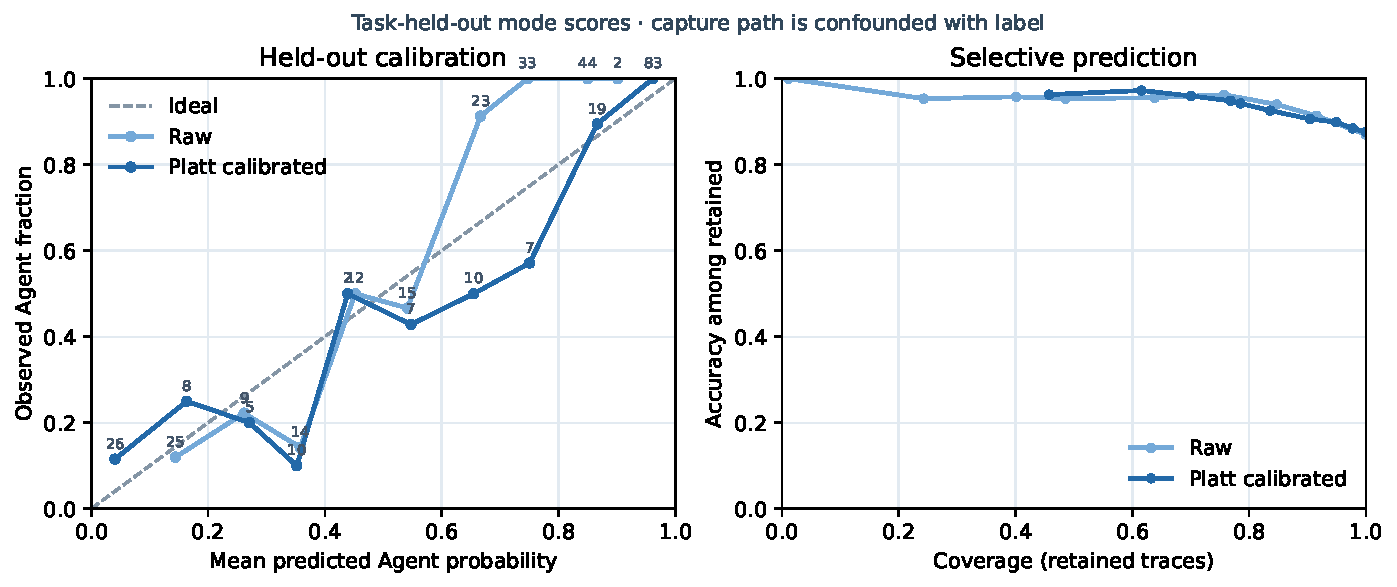
\includegraphics[width=\linewidth]{mixed_gallery_calibration.pdf}
\caption{Out-of-fold calibration and selective-prediction diagnostics. Scores describe Human/Agent record labels in the source release; capture path is confounded with the label.}
\label{fig:calibration}
\end{figure}

\paragraph{Pairwise error protocol.} The association-error experiment uses the same 177 traces and three benchmark-stratified outer task folds as the mixed-gallery study. Within each outer training partition, a second three-fold task-grouped cross-fit generates out-of-fold association scores for threshold selection. For each method, the threshold maximizes task-macro balanced accuracy over 101 empirical score quantiles and the observed score bounds; ties select the higher threshold. The outer test fold is scored once with the outer-training model and this fixed threshold. Pair features and pair-training labels are unchanged from the mixed-gallery rankers: benchmark/task identity constructs training positives and negatives, while the evaluator alone uses held-out task IDs.

For a query trace $q$, the false-split rate is the fraction of same-challenge candidates rejected, and the false-merge rate is the fraction of different-challenge candidates accepted. Candidate rates are averaged within each query, queries within each task, tasks within each benchmark, and benchmarks with equal weight. Task-macro balanced accuracy is $1 - (\mathrm{FNR}+\mathrm{FPR})/2$, where FNR and FPR denote these aggregated false-split and false-merge rates. The H--H, H--A, and A--A rates use the same query/task aggregation restricted to the indicated pair type. Pair rows are directed for query-level scoring; uncertainty resamples task groups, not pair rows.

The 95\% intervals use 5,000 paired task-cluster bootstrap samples within benchmark. Bootstrap draws condition on the fitted outer-fold models and the training-selected thresholds; they do not capture variability from repeating the complete nested fit. Pair-level outputs retain trace IDs, challenge-relevance labels, scores, and decisions; the worked-example JSON additionally includes allowlisted command names, but no raw logs, arguments, paths, or outputs. The reproducible implementation and figure code are in \texttt{scripts/run\_association\_error\_analysis.py}; the runnable notebook is \texttt{notebooks/08\_association\_error\_analysis.ipynb}.

\paragraph{Data source and license.} Cyber Task Horizons is pinned to commit \texttt{178c0da1800f9c07311e1b8d6c61dd8104e7b4ae} under CC BY 4.0. The manifest records selected source files, hashes, suite and task IDs, collection labels, and latest-attempt deduplication. Raw traces are fetched locally and are not redistributed by this repository. Task identity labels same-challenge retrieval relevance; shared intrusions are not annotated.

\paragraph{Reproduction.} From the repository root, install the locked CPU dependencies, download the pinned public traces, then run:

\begin{verbatim}
.venv/bin/python scripts/run_mixed_gallery.py --bootstraps 5000
.venv/bin/python scripts/run_association_error_analysis.py --bootstraps 5000 --threshold-grid 101
.venv/bin/python -m unittest discover -s tests -v
\end{verbatim}

The mixed-gallery run writes \texttt{results/mixed\_gallery.json}, task/query CSVs, held-out mode predictions, and three PDF/PNG figures. The association-error run writes \texttt{results/association\_error\_analysis.json}, pair-score, task-metric, and threshold CSVs, plus a PDF/PNG error-profile figure. Both result JSON files record the data revision, protocol version, evaluation definition, bootstrap method, and source hash. Figure-generation code remains in the corresponding experiment scripts.

\section{Follow-up feature and association protocol}

\paragraph{Feature ablation.} Four fixed inputs are compared: F0, log command count plus action proportions; F1, command-name TF--IDF unigrams and bigrams; F2, sequence transition, repetition, uniqueness, run-length, and short-trace statistics without command count; and F3, F1 concatenated with F2. Balanced logistic regression ($C=1$) and ExtraTrees (300 trees, depth 8, minimum leaf 3) are evaluated on six three-fold task-grouped splits. Vectorizers and models are fit only on training tasks. Estimates average each task across the six split seeds before a 5,000-draw benchmark-stratified task bootstrap. Repeated seeds are split-sensitivity checks, not independent replications.

\paragraph{Observation and order controls.} Prefix comparisons use matched task cohorts: 175 traces in 40 tasks for the two-command comparison, and 99 traces in 25 tasks for the four-command comparison. Full traces and prefixes are re-evaluated under the same task splits. On the four-command cohort, five fixed seeds shuffle aligned command/action events while preserving their counts. Paired intervals resample tasks within benchmark.

\paragraph{Model-source transfer.} Claude Opus, Claude Sonnet, and GPT-5.5 are each held out in turn. Tasks are also held out from training; test sets pair the held-out model's Agent traces with same-task Human records. Human test records recur across the three model panels, so the panels are dependent. This diagnoses model-source transfer on the current corpus rather than external validation.

\paragraph{Fixed-operating-point association.} The outer split uses three benchmark-stratified task folds with seed \texttt{20261030}. Each threshold is selected from inner task-held-out training predictions to minimize false splits subject to a task-macro false-merge ceiling of 10\%, 20\%, or 30\%. The 20\% ceiling is primary. Five methods share the same held-out candidates: command cosine, a behavior ranker containing command, action-bigram, ProcGrep, and length similarities, the behavior ranker plus fixed sequence statistics, the behavior ranker plus out-of-fold mode-agreement features, and a length-only control. Candidate inclusion is not conditioned on mode. Test false-merge rates are reported as observed and may differ from the training ceiling. Relevance is defined by the same CTF challenge. Results use 5,000 paired task-cluster bootstrap draws conditional on the fitted outer folds.

\paragraph{Audited worked examples.} Threshold examples C1--C3 are selected as the lexicographically first Human-query/Agent-candidate pairs in the recovered-link, introduced-link, and persistent-miss categories. Ranking example C4--C5 is selected from two held-out Human queries meeting a fixed criterion: behavior-only Hit@1 is zero, mode-aware Hit@1 is one, and at least one same-challenge Agent is tied at the top. In the selected InterCode-CTF query (trace \texttt{d209c425ee9ce2bf}; 39 candidates), behavior-only ranking puts the different-challenge Human trace \texttt{4cdc4644c4f559d9} first (score 0.6281) and the relevant Agent trace \texttt{1d9f0d5a2f0a520d} fifth (0.5800). Mode-aware ranking places the Agent first (0.6675) and the Human second (0.6605), changing query Hit@1 from 0 to 1. These are deliberately selected explanatory examples, not prevalence estimates. The extraction script independently refits the selected outer folds and verifies all frozen pair scores; the maximum absolute discrepancy is 0.0 and no task overlaps train and test. Full IDs, safe command-name previews, thresholds, scores, and ranks are in \texttt{results/association\_cases\_v1.json}. Figures are generated by \texttt{scripts/plot\_association\_cases.py}.

\paragraph{Reproduction.} With the pinned traces in the ignored \texttt{data/} directory, run:

\begin{verbatim}
.venv/bin/python scripts/run_feature_ablation.py
.venv/bin/python scripts/summarize_feature_contrasts.py
.venv/bin/python scripts/run_agent_model_transfer.py --bootstraps 5000
.venv/bin/python scripts/run_association_operating_points.py --bootstraps 5000 --threshold-grid 101
.venv/bin/python scripts/extract_association_cases.py --refit
.venv/bin/python scripts/plot_association_cases.py
.venv/bin/python scripts/plot_feature_ablation.py
.venv/bin/python scripts/plot_association_operating_points.py
\end{verbatim}

The feature and association notebooks are \texttt{notebooks/09\_feature\_ablation\_v1.ipynb} and \texttt{notebooks/10\_association\_operating\_points\_v1.ipynb}. Derived tables, predictions, thresholds, task-level scores, and figure-generation code are retained in \texttt{results/} and \texttt{scripts/}.
